%!TEX encoding = IsoLatin

%% Document is article 
\documentclass[a4paper]{article}

%% ----------------------------------------------------- PACKAGES ----------------------------------------------------- %%
\usepackage{coolArticle}

%% ---------------------------------------------------- DOCUMENT ---------------------------------------------------- %%
\begin{document}

\noindent \textsc{Gallos-Montbrun} Gr�goire\\
\textsc{Faury} Louis 
\vspace{15pt}

	\titlebox{0.6}{\Large Model Predictive Control}{\Large \textbf{\textcolor{blue}{Building Temperature Regulation}}}
	
	\section{Introduction}
	{
		\paragraph{} This project aims at controlling the temperature inside a 3 room building. The full state and output dynamics are given by : 
		\begin{equation}
			\begin{aligned}
				x^+ &= Ax + B_uu + B_dd\\
				y &= Cx
			\end{aligned}
		\end{equation}
		where : 
		\begin{equation}
		\left\{
			\begin{aligned}
				&x \in \mathbb{R}^{10} & &\text{ has no significant physical meaning} \\
				&u \in\mathbb{R}^3 & &\text{ is the electrical power dedicated to the heating of each room}\\
				&d \in\mathbb{R}^3 & &\text{ is the disturbance input (temperature, solar gain and internal gains)} \\
				&y\in\mathbb{R}^3 & & \text{ is the temperature in each room of the building}
			\end{aligned}\right.
		\end{equation}
		
		\paragraph{} The disturbance will be considered as an input, since we have its prediction over a period of 8 days. Figure (\ref{fig::temp_pred}) and (\ref{fig::gain_pred}) provide a plot of those predictive value. We can namely notice that we observe a \emph{\textcolor{red}{circadian periodicity}} (periodicity of 24h for the different signals). 
		
		\begin{figure}[h!]
			\begin{minipage}{0.45\linewidth}
				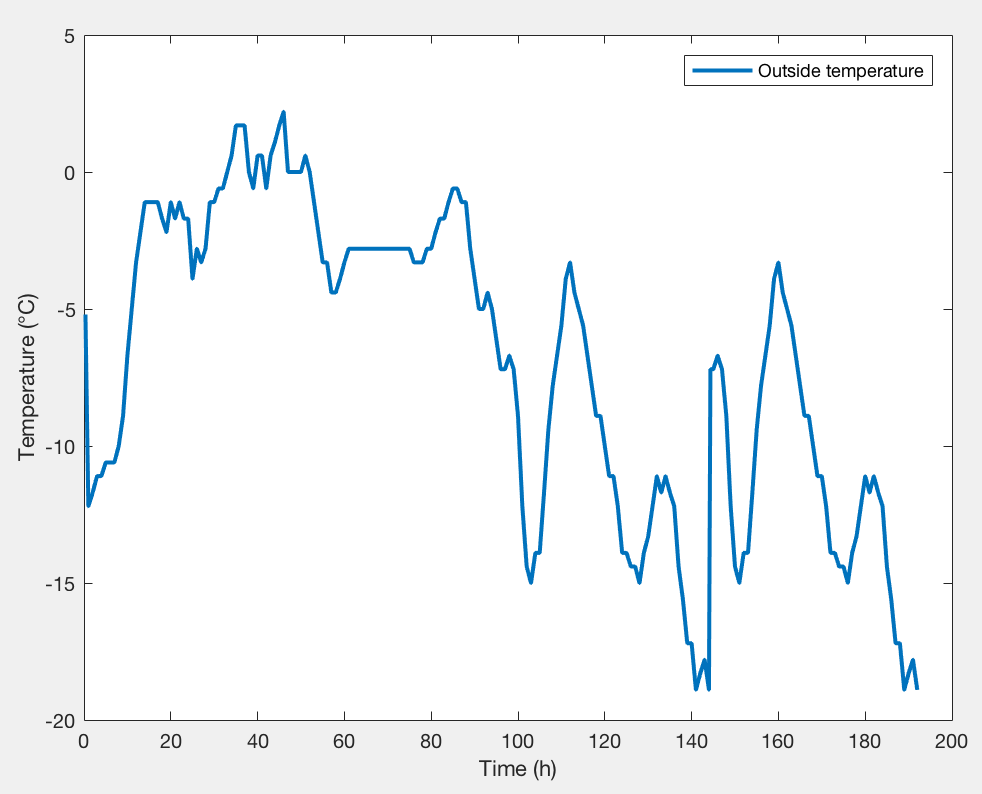
\includegraphics[width=\linewidth]{temp_pred}
				\caption{External temperature predictions}
				\label{fig::temp_pred}
			\end{minipage}
			\begin{minipage}{0.45\linewidth}
				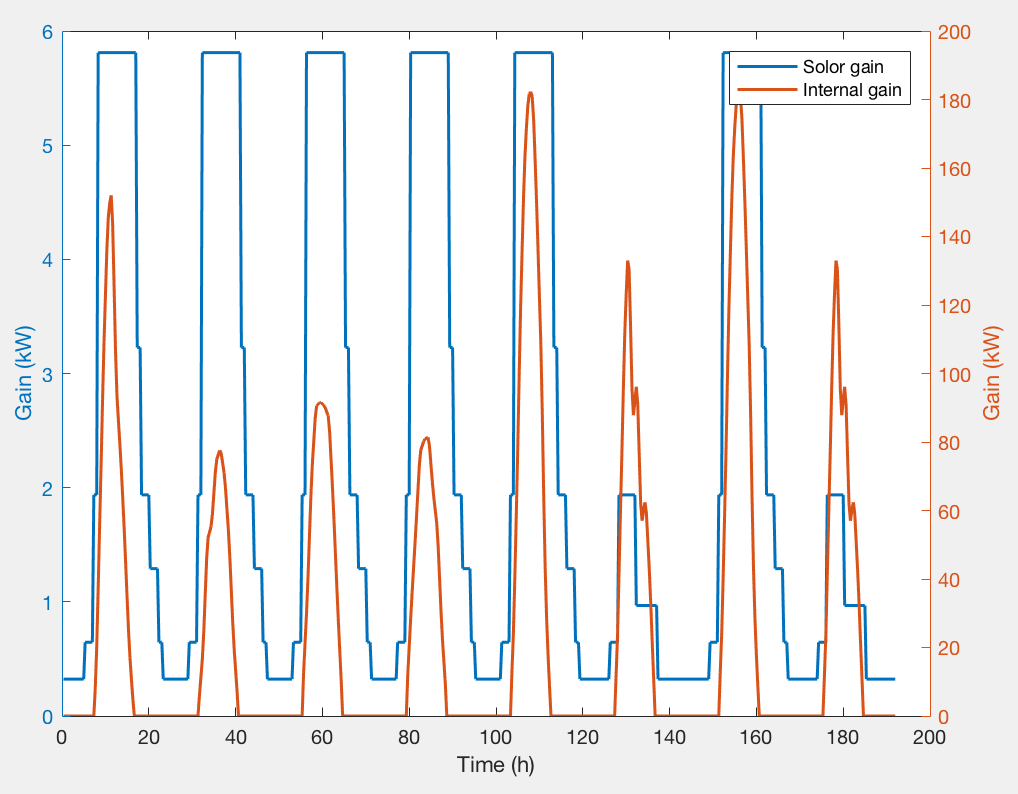
\includegraphics[width=\linewidth]{gains_pred}
				\caption{Solar and internal gain predictions}
				\label{fig::gain_pred}
			\end{minipage}
		\end{figure}
		
		\paragraph{} The following sections implements different versions of model predictive controllers, considering different objectives : target tracking, cost minimization, storage cost, .. 
	}
	
	\section{First MPC Controller}
	{
		\paragraph{} In this section, we are using YALMIP in order to design a MPC controller. This controller must regulate the output of the system around the reference output : 
		\begin{equation}
			y_r = \begin{pmatrix} 24 & 24 & 24 \end{pmatrix}
		\end{equation}
		by optimizing the cost function : 
		\begin{equation}
			J = \sum_{n=1}^N (y_n-y_r)^T R (y-y_n)
		\end{equation}
		In the following, $R$ is chosen to be $\mathds{1}_3$ (hence we are penalizing equally any fluctuations around the target value, independently of the room). We decided \emph{not to implement} a terminal cost nor terminal set constraints. This was mainly motivated by the fact that even with small horizons $N$, the system is \emph{experimentally} stable and recursively feasible. Hence, given the fact that the control invariant set could be computationally challenging to compute, and because we would highly reduce the attraction zone in our state space, there was no real need to use terminal cost or terminal set. 
		
		\paragraph{} % Display figures with different Ns, explain 
	}
   
\end{document}